\documentclass[1p]{elsarticle_modified}
%\bibliographystyle{elsarticle-num}

%\usepackage[colorlinks]{hyperref}
%\usepackage{abbrmath_seonhwa} %\Abb, \Ascr, \Acal ,\Abf, \Afrak
\usepackage{amsfonts}
\usepackage{amssymb}
\usepackage{amsmath}
\usepackage{amsthm}
\usepackage{scalefnt}
\usepackage{amsbsy}
\usepackage{kotex}
\usepackage{caption}
\usepackage{subfig}
\usepackage{color}
\usepackage{graphicx}
\usepackage{xcolor} %% white, black, red, green, blue, cyan, magenta, yellow
\usepackage{float}
\usepackage{setspace}
\usepackage{hyperref}

\usepackage{tikz}
\usetikzlibrary{arrows}

\usepackage{multirow}
\usepackage{array} % fixed length table
\usepackage{hhline}

%%%%%%%%%%%%%%%%%%%%%
\makeatletter
\renewcommand*\env@matrix[1][\arraystretch]{%
	\edef\arraystretch{#1}%
	\hskip -\arraycolsep
	\let\@ifnextchar\new@ifnextchar
	\array{*\c@MaxMatrixCols c}}
\makeatother %https://tex.stackexchange.com/questions/14071/how-can-i-increase-the-line-spacing-in-a-matrix
%%%%%%%%%%%%%%%

\usepackage[normalem]{ulem}

\newcommand{\msout}[1]{\ifmmode\text{\sout{\ensuremath{#1}}}\else\sout{#1}\fi}
%SOURCE: \msout is \stkout macro in https://tex.stackexchange.com/questions/20609/strikeout-in-math-mode

\newcommand{\cancel}[1]{
	\ifmmode
	{\color{red}\msout{#1}}
	\else
	{\color{red}\sout{#1}}
	\fi
}

\newcommand{\add}[1]{
	{\color{blue}\uwave{#1}}
}

\newcommand{\replace}[2]{
	\ifmmode
	{\color{red}\msout{#1}}{\color{blue}\uwave{#2}}
	\else
	{\color{red}\sout{#1}}{\color{blue}\uwave{#2}}
	\fi
}

\newcommand{\Sol}{\mathcal{S}} %segment
\newcommand{\D}{D} %diagram
\newcommand{\A}{\mathcal{A}} %arc


%%%%%%%%%%%%%%%%%%%%%%%%%%%%%5 test

\def\sl{\operatorname{\textup{SL}}(2,\Cbb)}
\def\psl{\operatorname{\textup{PSL}}(2,\Cbb)}
\def\quan{\mkern 1mu \triangleright \mkern 1mu}

\theoremstyle{definition}
\newtheorem{thm}{Theorem}[section]
\newtheorem{prop}[thm]{Proposition}
\newtheorem{lem}[thm]{Lemma}
\newtheorem{ques}[thm]{Question}
\newtheorem{cor}[thm]{Corollary}
\newtheorem{defn}[thm]{Definition}
\newtheorem{exam}[thm]{Example}
\newtheorem{rmk}[thm]{Remark}
\newtheorem{alg}[thm]{Algorithm}

\newcommand{\I}{\sqrt{-1}}
\begin{document}

%\begin{frontmatter}
%
%\title{Boundary parabolic representations of knots up to 8 crossings}
%
%%% Group authors per affiliation:
%\author{Yunhi Cho} 
%\address{Department of Mathematics, University of Seoul, Seoul, Korea}
%\ead{yhcho@uos.ac.kr}
%
%
%\author{Seonhwa Kim} %\fnref{s_kim}}
%\address{Center for Geometry and Physics, Institute for Basic Science, Pohang, 37673, Korea}
%\ead{ryeona17@ibs.re.kr}
%
%\author{Hyuk Kim}
%\address{Department of Mathematical Sciences, Seoul National University, Seoul 08826, Korea}
%\ead{hyukkim@snu.ac.kr}
%
%\author{Seokbeom Yoon}
%\address{Department of Mathematical Sciences, Seoul National University, Seoul, 08826,  Korea}
%\ead{sbyoon15@snu.ac.kr}
%
%\begin{abstract}
%We find all boundary parabolic representation of knots up to 8 crossings.
%
%\end{abstract}
%\begin{keyword}
%    \MSC[2010] 57M25 
%\end{keyword}
%
%\end{frontmatter}

%\linenumbers
%\tableofcontents
%
\newcommand\colored[1]{\textcolor{white}{\rule[-0.35ex]{0.8em}{1.4ex}}\kern-0.8em\color{red} #1}%
%\newcommand\colored[1]{\textcolor{white}{ #1}\kern-2.17ex	\textcolor{white}{ #1}\kern-1.81ex	\textcolor{white}{ #1}\kern-2.15ex\color{red}#1	}

{\Large $\underline{12a_{0214}~(K12a_{0214})}$}

\setlength{\tabcolsep}{10pt}
\renewcommand{\arraystretch}{1.6}
\vspace{1cm}\begin{tabular}{m{100pt}>{\centering\arraybackslash}m{274pt}}
\multirow{5}{120pt}{
	\centering
	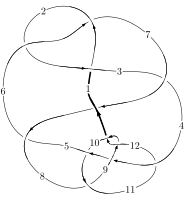
\includegraphics[width=112pt]{../../../GIT/diagram.site/Diagrams/png/1015_12a_0214.png}\\
\ \ \ A knot diagram\footnotemark}&
\allowdisplaybreaks
\textbf{Linearized knot diagam} \\
\cline{2-2}
 &
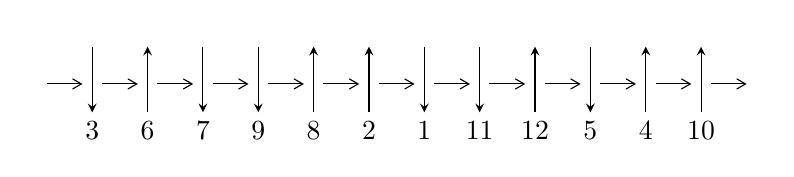
\begin{tikzpicture}[x=20pt, y=17pt]
	% nodes
	\node (C0) at (0, 0) {};
	\node (C1) at (1, 0) {};
	\node (C1U) at (1, +1) {};
	\node (C1D) at (1, -1) {3};

	\node (C2) at (2, 0) {};
	\node (C2U) at (2, +1) {};
	\node (C2D) at (2, -1) {6};

	\node (C3) at (3, 0) {};
	\node (C3U) at (3, +1) {};
	\node (C3D) at (3, -1) {7};

	\node (C4) at (4, 0) {};
	\node (C4U) at (4, +1) {};
	\node (C4D) at (4, -1) {9};

	\node (C5) at (5, 0) {};
	\node (C5U) at (5, +1) {};
	\node (C5D) at (5, -1) {8};

	\node (C6) at (6, 0) {};
	\node (C6U) at (6, +1) {};
	\node (C6D) at (6, -1) {2};

	\node (C7) at (7, 0) {};
	\node (C7U) at (7, +1) {};
	\node (C7D) at (7, -1) {1};

	\node (C8) at (8, 0) {};
	\node (C8U) at (8, +1) {};
	\node (C8D) at (8, -1) {11};

	\node (C9) at (9, 0) {};
	\node (C9U) at (9, +1) {};
	\node (C9D) at (9, -1) {12};

	\node (C10) at (10, 0) {};
	\node (C10U) at (10, +1) {};
	\node (C10D) at (10, -1) {5};

	\node (C11) at (11, 0) {};
	\node (C11U) at (11, +1) {};
	\node (C11D) at (11, -1) {4};

	\node (C12) at (12, 0) {};
	\node (C12U) at (12, +1) {};
	\node (C12D) at (12, -1) {10};
	\node (C13) at (13, 0) {};

	% arrows
	\draw[->,>={angle 60}]
	(C0) edge (C1) (C1) edge (C2) (C2) edge (C3) (C3) edge (C4) (C4) edge (C5) (C5) edge (C6) (C6) edge (C7) (C7) edge (C8) (C8) edge (C9) (C9) edge (C10) (C10) edge (C11) (C11) edge (C12) (C12) edge (C13) ;	\draw[->,>=stealth]
	(C1U) edge (C1D) (C2D) edge (C2U) (C3U) edge (C3D) (C4U) edge (C4D) (C5D) edge (C5U) (C6D) edge (C6U) (C7U) edge (C7D) (C8U) edge (C8D) (C9D) edge (C9U) (C10U) edge (C10D) (C11D) edge (C11U) (C12D) edge (C12U) ;
	\end{tikzpicture} \\
\hhline{~~} \\& 
\textbf{Solving Sequence} \\ \cline{2-2} 
 &
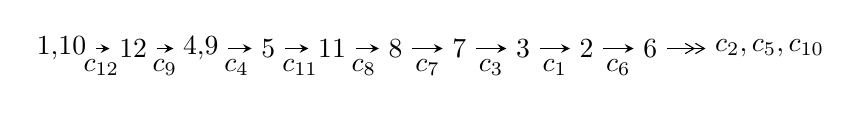
\begin{tikzpicture}[x=23pt, y=7pt]
	% node
	\node (A0) at (-1/8, 0) {1,10};
	\node (A1) at (1, 0) {12};
	\node (A2) at (33/16, 0) {4,9};
	\node (A3) at (25/8, 0) {5};
	\node (A4) at (33/8, 0) {11};
	\node (A5) at (41/8, 0) {8};
	\node (A6) at (49/8, 0) {7};
	\node (A7) at (57/8, 0) {3};
	\node (A8) at (65/8, 0) {2};
	\node (A9) at (73/8, 0) {6};
	\node (C1) at (1/2, -1) {$c_{12}$};
	\node (C2) at (3/2, -1) {$c_{9}$};
	\node (C3) at (21/8, -1) {$c_{4}$};
	\node (C4) at (29/8, -1) {$c_{11}$};
	\node (C5) at (37/8, -1) {$c_{8}$};
	\node (C6) at (45/8, -1) {$c_{7}$};
	\node (C7) at (53/8, -1) {$c_{3}$};
	\node (C8) at (61/8, -1) {$c_{1}$};
	\node (C9) at (69/8, -1) {$c_{6}$};
	\node (A10) at (11, 0) {$c_{2},c_{5},c_{10}$};

	% edge
	\draw[->,>=stealth]	
	(A0) edge (A1) (A1) edge (A2) (A2) edge (A3) (A3) edge (A4) (A4) edge (A5) (A5) edge (A6) (A6) edge (A7) (A7) edge (A8) (A8) edge (A9) ;
	\draw[->>,>={angle 60}]	
	(A9) edge (A10);
\end{tikzpicture} \\ 

\end{tabular} \\

\footnotetext{
The image of knot diagram is generated by the software ``\textbf{Draw programme}" developed by Andrew Bartholomew(\url{http://www.layer8.co.uk/maths/draw/index.htm\#Running-draw}), where we modified some parts for our purpose(\url{https://github.com/CATsTAILs/LinksPainter}).
}\phantom \\ \newline 
\centering \textbf{Ideals for irreducible components\footnotemark of $X_{\text{par}}$} 
 
\begin{align*}
I^u_{1}&=\langle 
1.93994\times10^{450} u^{129}+4.30877\times10^{450} u^{128}+\cdots+4.13780\times10^{449} b+1.94502\times10^{450},\\
\phantom{I^u_{1}}&\phantom{= \langle  }6.48985\times10^{449} u^{129}+1.44403\times10^{450} u^{128}+\cdots+2.06890\times10^{449} a+4.51017\times10^{449},\;u^{130}+3 u^{129}+\cdots+6 u+1\rangle \\
I^u_{2}&=\langle 
b^2- b+1,\;a-1,\;u-1\rangle \\
\\
\end{align*}
\raggedright * 2 irreducible components of $\dim_{\mathbb{C}}=0$, with total 132 representations.\\
\footnotetext{All coefficients of polynomials are rational numbers. But the coefficients are sometimes approximated in decimal forms when there is not enough margin.}
\newpage
\renewcommand{\arraystretch}{1}
\centering \section*{I. $I^u_{1}= \langle 1.94\times10^{450} u^{129}+4.31\times10^{450} u^{128}+\cdots+4.14\times10^{449} b+1.95\times10^{450},\;6.49\times10^{449} u^{129}+1.44\times10^{450} u^{128}+\cdots+2.07\times10^{449} a+4.51\times10^{449},\;u^{130}+3 u^{129}+\cdots+6 u+1 \rangle$}
\flushleft \textbf{(i) Arc colorings}\\
\begin{tabular}{m{7pt} m{180pt} m{7pt} m{180pt} }
\flushright $a_{1}=$&$\begin{pmatrix}1\\0\end{pmatrix}$ \\
\flushright $a_{10}=$&$\begin{pmatrix}0\\u\end{pmatrix}$ \\
\flushright $a_{12}=$&$\begin{pmatrix}1\\u^2\end{pmatrix}$ \\
\flushright $a_{4}=$&$\begin{pmatrix}-3.13686 u^{129}-6.97970 u^{128}+\cdots-0.718419 u-2.17998\\-4.68833 u^{129}-10.4132 u^{128}+\cdots-25.8623 u-4.70060\end{pmatrix}$ \\
\flushright $a_{9}=$&$\begin{pmatrix}- u\\- u^3+u\end{pmatrix}$ \\
\flushright $a_{5}=$&$\begin{pmatrix}0.688229 u^{129}+1.91659 u^{128}+\cdots+23.5319 u+2.80523\\-6.83080 u^{129}-15.1988 u^{128}+\cdots-38.4640 u-7.10686\end{pmatrix}$ \\
\flushright $a_{11}=$&$\begin{pmatrix}-0.178952 u^{129}-0.322850 u^{128}+\cdots-15.4701 u-2.97465\\-0.203119 u^{129}-0.342260 u^{128}+\cdots+3.55349 u-0.286047\end{pmatrix}$ \\
\flushright $a_{8}=$&$\begin{pmatrix}-0.127207 u^{129}-0.274547 u^{128}+\cdots-3.51528 u-1.21382\\0.126131 u^{129}+0.262206 u^{128}+\cdots+3.00004 u+0.106749\end{pmatrix}$ \\
\flushright $a_{7}=$&$\begin{pmatrix}-0.00107554 u^{129}-0.0123410 u^{128}+\cdots-0.515235 u-1.10707\\0.126131 u^{129}+0.262206 u^{128}+\cdots+3.00004 u+0.106749\end{pmatrix}$ \\
\flushright $a_{3}=$&$\begin{pmatrix}-1.80077 u^{129}-3.86071 u^{128}+\cdots+2.72723 u-1.64091\\-1.70303 u^{129}-3.14021 u^{128}+\cdots-10.6563 u-1.80268\end{pmatrix}$ \\
\flushright $a_{2}=$&$\begin{pmatrix}-0.417240 u^{129}-1.50730 u^{128}+\cdots-28.9400 u-3.28010\\0.0678887 u^{129}-0.183675 u^{128}+\cdots+3.18011 u-0.444522\end{pmatrix}$ \\
\flushright $a_{6}=$&$\begin{pmatrix}-3.06909 u^{129}-6.85322 u^{128}+\cdots-4.64774 u-3.01184\\-2.12072 u^{129}-4.95178 u^{128}+\cdots-12.9002 u-2.74315\end{pmatrix}$\\&\end{tabular}
\flushleft \textbf{(ii) Obstruction class $= -1$}\\~\\
\flushleft \textbf{(iii) Cusp Shapes $= 8.59696 u^{129}+20.3475 u^{128}+\cdots+46.5185 u+8.91533$}\\~\\
\newpage\renewcommand{\arraystretch}{1}
\flushleft \textbf{(iv) u-Polynomials at the component}\newline \\
\begin{tabular}{m{50pt}|m{274pt}}
Crossings & \hspace{64pt}u-Polynomials at each crossing \\
\hline $$\begin{aligned}c_{1}\end{aligned}$$&$\begin{aligned}
&u^{130}+62 u^{129}+\cdots+5 u+1
\end{aligned}$\\
\hline $$\begin{aligned}c_{2},c_{6}\end{aligned}$$&$\begin{aligned}
&u^{130}-2 u^{129}+\cdots-5 u+1
\end{aligned}$\\
\hline $$\begin{aligned}c_{3}\end{aligned}$$&$\begin{aligned}
&u^{130}+2 u^{129}+\cdots+41643 u+4113
\end{aligned}$\\
\hline $$\begin{aligned}c_{4}\end{aligned}$$&$\begin{aligned}
&u^{130}+4 u^{129}+\cdots+u+1
\end{aligned}$\\
\hline $$\begin{aligned}c_{5}\end{aligned}$$&$\begin{aligned}
&u^{130}+14 u^{129}+\cdots-2746727 u+111833
\end{aligned}$\\
\hline $$\begin{aligned}c_{7}\end{aligned}$$&$\begin{aligned}
&u^{130}-5 u^{129}+\cdots-58912 u+6976
\end{aligned}$\\
\hline $$\begin{aligned}c_{8}\end{aligned}$$&$\begin{aligned}
&u^{130}-21 u^{129}+\cdots-12 u+4
\end{aligned}$\\
\hline $$\begin{aligned}c_{9},c_{12}\end{aligned}$$&$\begin{aligned}
&u^{130}+3 u^{129}+\cdots+6 u+1
\end{aligned}$\\
\hline $$\begin{aligned}c_{10}\end{aligned}$$&$\begin{aligned}
&u^{130}-2 u^{129}+\cdots-19 u+1
\end{aligned}$\\
\hline $$\begin{aligned}c_{11}\end{aligned}$$&$\begin{aligned}
&u^{130}-4 u^{129}+\cdots-1271 u+131
\end{aligned}$\\
\hline
\end{tabular}\\~\\
\newpage\renewcommand{\arraystretch}{1}
\flushleft \textbf{(v) Riley Polynomials at the component}\newline \\
\begin{tabular}{m{50pt}|m{274pt}}
Crossings & \hspace{64pt}Riley Polynomials at each crossing \\
\hline $$\begin{aligned}c_{1}\end{aligned}$$&$\begin{aligned}
&y^{130}+14 y^{129}+\cdots+97 y+1
\end{aligned}$\\
\hline $$\begin{aligned}c_{2},c_{6}\end{aligned}$$&$\begin{aligned}
&y^{130}+62 y^{129}+\cdots+5 y+1
\end{aligned}$\\
\hline $$\begin{aligned}c_{3}\end{aligned}$$&$\begin{aligned}
&y^{130}-34 y^{129}+\cdots-460845135 y+16916769
\end{aligned}$\\
\hline $$\begin{aligned}c_{4}\end{aligned}$$&$\begin{aligned}
&y^{130}+22 y^{129}+\cdots+5 y+1
\end{aligned}$\\
\hline $$\begin{aligned}c_{5}\end{aligned}$$&$\begin{aligned}
&y^{130}+50 y^{129}+\cdots-7595894910367 y+12506619889
\end{aligned}$\\
\hline $$\begin{aligned}c_{7}\end{aligned}$$&$\begin{aligned}
&y^{130}+17 y^{129}+\cdots+4190851968 y+48664576
\end{aligned}$\\
\hline $$\begin{aligned}c_{8}\end{aligned}$$&$\begin{aligned}
&y^{130}-15 y^{129}+\cdots-360 y+16
\end{aligned}$\\
\hline $$\begin{aligned}c_{9},c_{12}\end{aligned}$$&$\begin{aligned}
&y^{130}-81 y^{129}+\cdots+30 y+1
\end{aligned}$\\
\hline $$\begin{aligned}c_{10}\end{aligned}$$&$\begin{aligned}
&y^{130}-118 y^{129}+\cdots+121 y+1
\end{aligned}$\\
\hline $$\begin{aligned}c_{11}\end{aligned}$$&$\begin{aligned}
&y^{130}-130 y^{129}+\cdots-1175543 y+17161
\end{aligned}$\\
\hline
\end{tabular}\\~\\
\newpage\flushleft \textbf{(vi) Complex Volumes and Cusp Shapes}
$$\begin{array}{c|c|c}  
\text{Solutions to }I^u_{1}& \I (\text{vol} + \sqrt{-1}CS) & \text{Cusp shape}\\
 \hline 
\begin{aligned}
u &= \phantom{-}0.749532 + 0.664227 I \\
a &= -0.871953 + 0.384851 I \\
b &= \phantom{-}0.502067 - 0.431748 I\end{aligned}
 & \phantom{-}1.95298 + 0.77909 I & \phantom{-0.000000 } 0 \\ \hline\begin{aligned}
u &= \phantom{-}0.749532 - 0.664227 I \\
a &= -0.871953 - 0.384851 I \\
b &= \phantom{-}0.502067 + 0.431748 I\end{aligned}
 & \phantom{-}1.95298 - 0.77909 I & \phantom{-0.000000 } 0 \\ \hline\begin{aligned}
u &= \phantom{-}0.961298 + 0.290000 I \\
a &= -1.080940 + 0.022623 I \\
b &= \phantom{-}0.0561571 + 0.0027518 I\end{aligned}
 & \phantom{-}1.86525 + 0.92233 I & \phantom{-0.000000 } 0 \\ \hline\begin{aligned}
u &= \phantom{-}0.961298 - 0.290000 I \\
a &= -1.080940 - 0.022623 I \\
b &= \phantom{-}0.0561571 - 0.0027518 I\end{aligned}
 & \phantom{-}1.86525 - 0.92233 I & \phantom{-0.000000 } 0 \\ \hline\begin{aligned}
u &= \phantom{-}0.997565 + 0.149599 I \\
a &= -3.28445 - 0.12377 I \\
b &= -0.374638 - 1.113690 I\end{aligned}
 & -2.60529 + 0.52783 I & \phantom{-0.000000 } 0 \\ \hline\begin{aligned}
u &= \phantom{-}0.997565 - 0.149599 I \\
a &= -3.28445 + 0.12377 I \\
b &= -0.374638 + 1.113690 I\end{aligned}
 & -2.60529 - 0.52783 I & \phantom{-0.000000 } 0 \\ \hline\begin{aligned}
u &= -0.968506 + 0.163873 I \\
a &= -2.16914 + 0.57550 I \\
b &= -1.45050 + 1.08479 I\end{aligned}
 & \phantom{-}1.75057 + 1.14387 I & \phantom{-0.000000 } 0 \\ \hline\begin{aligned}
u &= -0.968506 - 0.163873 I \\
a &= -2.16914 - 0.57550 I \\
b &= -1.45050 - 1.08479 I\end{aligned}
 & \phantom{-}1.75057 - 1.14387 I & \phantom{-0.000000 } 0 \\ \hline\begin{aligned}
u &= -0.995720 + 0.222833 I \\
a &= \phantom{-}2.03831 - 0.62029 I \\
b &= \phantom{-}1.25938 - 1.29158 I\end{aligned}
 & \phantom{-}2.64549 - 3.86577 I & \phantom{-0.000000 } 0 \\ \hline\begin{aligned}
u &= -0.995720 - 0.222833 I \\
a &= \phantom{-}2.03831 + 0.62029 I \\
b &= \phantom{-}1.25938 + 1.29158 I\end{aligned}
 & \phantom{-}2.64549 + 3.86577 I & \phantom{-0.000000 } 0\\
 \hline 
 \end{array}$$\newpage$$\begin{array}{c|c|c}  
\text{Solutions to }I^u_{1}& \I (\text{vol} + \sqrt{-1}CS) & \text{Cusp shape}\\
 \hline 
\begin{aligned}
u &= -0.253514 + 0.997845 I \\
a &= -0.351240 + 0.216973 I \\
b &= -0.076787 - 0.822116 I\end{aligned}
 & -3.08998 + 1.62477 I & \phantom{-0.000000 } 0 \\ \hline\begin{aligned}
u &= -0.253514 - 0.997845 I \\
a &= -0.351240 - 0.216973 I \\
b &= -0.076787 + 0.822116 I\end{aligned}
 & -3.08998 - 1.62477 I & \phantom{-0.000000 } 0 \\ \hline\begin{aligned}
u &= -0.977192 + 0.341390 I \\
a &= -1.85611 + 0.59447 I \\
b &= -0.79872 + 1.39391 I\end{aligned}
 & -3.64756 - 3.52766 I & \phantom{-0.000000 } 0 \\ \hline\begin{aligned}
u &= -0.977192 - 0.341390 I \\
a &= -1.85611 - 0.59447 I \\
b &= -0.79872 - 1.39391 I\end{aligned}
 & -3.64756 + 3.52766 I & \phantom{-0.000000 } 0 \\ \hline\begin{aligned}
u &= \phantom{-}1.034360 + 0.075510 I \\
a &= \phantom{-}3.53031 - 0.10655 I \\
b &= \phantom{-}0.669756 + 0.640893 I\end{aligned}
 & \phantom{-}2.83600 + 1.66368 I & \phantom{-0.000000 } 0 \\ \hline\begin{aligned}
u &= \phantom{-}1.034360 - 0.075510 I \\
a &= \phantom{-}3.53031 + 0.10655 I \\
b &= \phantom{-}0.669756 - 0.640893 I\end{aligned}
 & \phantom{-}2.83600 - 1.66368 I & \phantom{-0.000000 } 0 \\ \hline\begin{aligned}
u &= \phantom{-}1.030110 + 0.130980 I \\
a &= \phantom{-}3.41041 + 0.07777 I \\
b &= \phantom{-}0.609353 + 1.033790 I\end{aligned}
 & \phantom{-}1.61147 + 3.27657 I & \phantom{-0.000000 } 0 \\ \hline\begin{aligned}
u &= \phantom{-}1.030110 - 0.130980 I \\
a &= \phantom{-}3.41041 - 0.07777 I \\
b &= \phantom{-}0.609353 - 1.033790 I\end{aligned}
 & \phantom{-}1.61147 - 3.27657 I & \phantom{-0.000000 } 0 \\ \hline\begin{aligned}
u &= \phantom{-}0.328696 + 0.898113 I \\
a &= \phantom{-}0.420332 - 0.284612 I \\
b &= -1.007830 - 0.093419 I\end{aligned}
 & \phantom{-}0.60196 + 6.82261 I & \phantom{-0.000000 } 0 \\ \hline\begin{aligned}
u &= \phantom{-}0.328696 - 0.898113 I \\
a &= \phantom{-}0.420332 + 0.284612 I \\
b &= -1.007830 + 0.093419 I\end{aligned}
 & \phantom{-}0.60196 - 6.82261 I & \phantom{-0.000000 } 0\\
 \hline 
 \end{array}$$\newpage$$\begin{array}{c|c|c}  
\text{Solutions to }I^u_{1}& \I (\text{vol} + \sqrt{-1}CS) & \text{Cusp shape}\\
 \hline 
\begin{aligned}
u &= \phantom{-}1.038030 + 0.147285 I \\
a &= -3.42187 - 0.13699 I \\
b &= -0.642604 - 1.156970 I\end{aligned}
 & -0.71281 + 8.13527 I & \phantom{-0.000000 } 0 \\ \hline\begin{aligned}
u &= \phantom{-}1.038030 - 0.147285 I \\
a &= -3.42187 + 0.13699 I \\
b &= -0.642604 + 1.156970 I\end{aligned}
 & -0.71281 - 8.13527 I & \phantom{-0.000000 } 0 \\ \hline\begin{aligned}
u &= -0.000698 + 1.049920 I \\
a &= \phantom{-}0.0343799 + 0.0694135 I \\
b &= -0.762613 - 0.819135 I\end{aligned}
 & -0.76360 + 1.63337 I & \phantom{-0.000000 } 0 \\ \hline\begin{aligned}
u &= -0.000698 - 1.049920 I \\
a &= \phantom{-}0.0343799 - 0.0694135 I \\
b &= -0.762613 + 0.819135 I\end{aligned}
 & -0.76360 - 1.63337 I & \phantom{-0.000000 } 0 \\ \hline\begin{aligned}
u &= \phantom{-}1.052110 + 0.040289 I \\
a &= -3.70281 + 0.10225 I \\
b &= -0.802349 - 0.356302 I\end{aligned}
 & \phantom{-}1.64097 - 2.69111 I & \phantom{-0.000000 } 0 \\ \hline\begin{aligned}
u &= \phantom{-}1.052110 - 0.040289 I \\
a &= -3.70281 - 0.10225 I \\
b &= -0.802349 + 0.356302 I\end{aligned}
 & \phantom{-}1.64097 + 2.69111 I & \phantom{-0.000000 } 0 \\ \hline\begin{aligned}
u &= -0.308603 + 1.013000 I \\
a &= \phantom{-}0.406602 - 0.292542 I \\
b &= -0.087122 + 0.849118 I\end{aligned}
 & -5.67692 - 2.95307 I & \phantom{-0.000000 } 0 \\ \hline\begin{aligned}
u &= -0.308603 - 1.013000 I \\
a &= \phantom{-}0.406602 + 0.292542 I \\
b &= -0.087122 - 0.849118 I\end{aligned}
 & -5.67692 + 2.95307 I & \phantom{-0.000000 } 0 \\ \hline\begin{aligned}
u &= -1.028110 + 0.311386 I \\
a &= \phantom{-}1.90194 - 0.65942 I \\
b &= \phantom{-}0.97779 - 1.54127 I\end{aligned}
 & \phantom{-}1.09535 - 6.30085 I & \phantom{-0.000000 } 0 \\ \hline\begin{aligned}
u &= -1.028110 - 0.311386 I \\
a &= \phantom{-}1.90194 + 0.65942 I \\
b &= \phantom{-}0.97779 + 1.54127 I\end{aligned}
 & \phantom{-}1.09535 + 6.30085 I & \phantom{-0.000000 } 0\\
 \hline 
 \end{array}$$\newpage$$\begin{array}{c|c|c}  
\text{Solutions to }I^u_{1}& \I (\text{vol} + \sqrt{-1}CS) & \text{Cusp shape}\\
 \hline 
\begin{aligned}
u &= -1.044560 + 0.333444 I \\
a &= -1.87493 + 0.68078 I \\
b &= -0.91797 + 1.63411 I\end{aligned}
 & -1.24102 - 11.41750 I & \phantom{-0.000000 } 0 \\ \hline\begin{aligned}
u &= -1.044560 - 0.333444 I \\
a &= -1.87493 - 0.68078 I \\
b &= -0.91797 - 1.63411 I\end{aligned}
 & -1.24102 + 11.41750 I & \phantom{-0.000000 } 0 \\ \hline\begin{aligned}
u &= \phantom{-}0.883723 + 0.167045 I \\
a &= \phantom{-}2.90602 + 0.27453 I \\
b &= -0.223286 + 1.021670 I\end{aligned}
 & -2.88331 + 0.66419 I & \phantom{-0.000000 } 0 \\ \hline\begin{aligned}
u &= \phantom{-}0.883723 - 0.167045 I \\
a &= \phantom{-}2.90602 - 0.27453 I \\
b &= -0.223286 - 1.021670 I\end{aligned}
 & -2.88331 - 0.66419 I & \phantom{-0.000000 } 0 \\ \hline\begin{aligned}
u &= -0.247591 + 1.073740 I \\
a &= \phantom{-}0.269586 - 0.308543 I \\
b &= \phantom{-}0.089589 + 1.050060 I\end{aligned}
 & -6.93321 + 4.86901 I & \phantom{-0.000000 } 0 \\ \hline\begin{aligned}
u &= -0.247591 - 1.073740 I \\
a &= \phantom{-}0.269586 + 0.308543 I \\
b &= \phantom{-}0.089589 - 1.050060 I\end{aligned}
 & -6.93321 - 4.86901 I & \phantom{-0.000000 } 0 \\ \hline\begin{aligned}
u &= \phantom{-}0.390854 + 0.791811 I \\
a &= -0.504519 + 0.425158 I \\
b &= \phantom{-}0.866825 - 0.042954 I\end{aligned}
 & \phantom{-}2.26305 + 2.23337 I & \phantom{-0.000000 } 0 \\ \hline\begin{aligned}
u &= \phantom{-}0.390854 - 0.791811 I \\
a &= -0.504519 - 0.425158 I \\
b &= \phantom{-}0.866825 + 0.042954 I\end{aligned}
 & \phantom{-}2.26305 - 2.23337 I & \phantom{-0.000000 } 0 \\ \hline\begin{aligned}
u &= -0.044947 + 1.123350 I \\
a &= -0.030537 - 0.197904 I \\
b &= \phantom{-}0.740708 + 1.064570 I\end{aligned}
 & \phantom{-}0.01779 + 6.20260 I & \phantom{-0.000000 } 0 \\ \hline\begin{aligned}
u &= -0.044947 - 1.123350 I \\
a &= -0.030537 + 0.197904 I \\
b &= \phantom{-}0.740708 - 1.064570 I\end{aligned}
 & \phantom{-}0.01779 - 6.20260 I & \phantom{-0.000000 } 0\\
 \hline 
 \end{array}$$\newpage$$\begin{array}{c|c|c}  
\text{Solutions to }I^u_{1}& \I (\text{vol} + \sqrt{-1}CS) & \text{Cusp shape}\\
 \hline 
\begin{aligned}
u &= -0.748193 + 0.441462 I \\
a &= \phantom{-}1.61678 - 0.31198 I \\
b &= \phantom{-}0.288025 - 0.755850 I\end{aligned}
 & -5.43884 - 3.19405 I & \phantom{-0.000000 } 0 \\ \hline\begin{aligned}
u &= -0.748193 - 0.441462 I \\
a &= \phantom{-}1.61678 + 0.31198 I \\
b &= \phantom{-}0.288025 + 0.755850 I\end{aligned}
 & -5.43884 + 3.19405 I & \phantom{-0.000000 } 0 \\ \hline\begin{aligned}
u &= -0.773867 + 0.390257 I \\
a &= \phantom{-}0.277986 + 0.438230 I \\
b &= \phantom{-}0.056039 + 1.165640 I\end{aligned}
 & -4.26513 - 8.43825 I & \phantom{-0.000000 } 0 \\ \hline\begin{aligned}
u &= -0.773867 - 0.390257 I \\
a &= \phantom{-}0.277986 - 0.438230 I \\
b &= \phantom{-}0.056039 - 1.165640 I\end{aligned}
 & -4.26513 + 8.43825 I & \phantom{-0.000000 } 0 \\ \hline\begin{aligned}
u &= -0.852307 + 0.061470 I \\
a &= -0.210768 - 1.318300 I \\
b &= -0.18942 - 1.68517 I\end{aligned}
 & \phantom{-}1.10773 - 2.44446 I & \phantom{-0.000000 } 0 \\ \hline\begin{aligned}
u &= -0.852307 - 0.061470 I \\
a &= -0.210768 + 1.318300 I \\
b &= -0.18942 + 1.68517 I\end{aligned}
 & \phantom{-}1.10773 + 2.44446 I & \phantom{-0.000000 } 0 \\ \hline\begin{aligned}
u &= \phantom{-}0.818290 + 0.804472 I \\
a &= \phantom{-}0.850507 - 0.315048 I \\
b &= -0.587697 + 0.724409 I\end{aligned}
 & -0.23288 - 3.80920 I & \phantom{-0.000000 } 0 \\ \hline\begin{aligned}
u &= \phantom{-}0.818290 - 0.804472 I \\
a &= \phantom{-}0.850507 + 0.315048 I \\
b &= -0.587697 - 0.724409 I\end{aligned}
 & -0.23288 + 3.80920 I & \phantom{-0.000000 } 0 \\ \hline\begin{aligned}
u &= \phantom{-}0.812762 + 0.193755 I \\
a &= \phantom{-}2.77598 + 0.45380 I \\
b &= -0.531184 + 0.968139 I\end{aligned}
 & -1.23884 - 6.87227 I & \phantom{-0.000000 } 0 \\ \hline\begin{aligned}
u &= \phantom{-}0.812762 - 0.193755 I \\
a &= \phantom{-}2.77598 - 0.45380 I \\
b &= -0.531184 - 0.968139 I\end{aligned}
 & -1.23884 + 6.87227 I & \phantom{-0.000000 } 0\\
 \hline 
 \end{array}$$\newpage$$\begin{array}{c|c|c}  
\text{Solutions to }I^u_{1}& \I (\text{vol} + \sqrt{-1}CS) & \text{Cusp shape}\\
 \hline 
\begin{aligned}
u &= -0.770981 + 0.321204 I \\
a &= -0.267104 - 0.610922 I \\
b &= -0.144345 - 1.229580 I\end{aligned}
 & -1.57828 - 3.67286 I & \phantom{-0.000000 } 0 \\ \hline\begin{aligned}
u &= -0.770981 - 0.321204 I \\
a &= -0.267104 + 0.610922 I \\
b &= -0.144345 + 1.229580 I\end{aligned}
 & -1.57828 + 3.67286 I & \phantom{-0.000000 } 0 \\ \hline\begin{aligned}
u &= \phantom{-}0.809501 + 0.148398 I \\
a &= -2.68553 - 0.36658 I \\
b &= \phantom{-}0.447773 - 0.823256 I\end{aligned}
 & \phantom{-}1.08788 - 2.14422 I & \phantom{-0.000000 } 0 \\ \hline\begin{aligned}
u &= \phantom{-}0.809501 - 0.148398 I \\
a &= -2.68553 + 0.36658 I \\
b &= \phantom{-}0.447773 + 0.823256 I\end{aligned}
 & \phantom{-}1.08788 + 2.14422 I & \phantom{-0.000000 } 0 \\ \hline\begin{aligned}
u &= -0.612842 + 0.542603 I \\
a &= \phantom{-}1.374370 - 0.173773 I \\
b &= \phantom{-}0.053565 - 0.427204 I\end{aligned}
 & -4.66525 + 4.55914 I & \phantom{-0.000000 } 0 \\ \hline\begin{aligned}
u &= -0.612842 - 0.542603 I \\
a &= \phantom{-}1.374370 + 0.173773 I \\
b &= \phantom{-}0.053565 + 0.427204 I\end{aligned}
 & -4.66525 - 4.55914 I & \phantom{-0.000000 } 0 \\ \hline\begin{aligned}
u &= -0.140788 + 1.173940 I \\
a &= -0.047975 + 0.337395 I \\
b &= -0.49629 - 1.33236 I\end{aligned}
 & -6.04376 + 5.27226 I & \phantom{-0.000000 } 0 \\ \hline\begin{aligned}
u &= -0.140788 - 1.173940 I \\
a &= -0.047975 - 0.337395 I \\
b &= -0.49629 + 1.33236 I\end{aligned}
 & -6.04376 - 5.27226 I & \phantom{-0.000000 } 0 \\ \hline\begin{aligned}
u &= -0.096709 + 1.190760 I \\
a &= -0.019172 - 0.321659 I \\
b &= \phantom{-}0.66614 + 1.34067 I\end{aligned}
 & -1.57307 + 8.12778 I & \phantom{-0.000000 } 0 \\ \hline\begin{aligned}
u &= -0.096709 - 1.190760 I \\
a &= -0.019172 + 0.321659 I \\
b &= \phantom{-}0.66614 - 1.34067 I\end{aligned}
 & -1.57307 - 8.12778 I & \phantom{-0.000000 } 0\\
 \hline 
 \end{array}$$\newpage$$\begin{array}{c|c|c}  
\text{Solutions to }I^u_{1}& \I (\text{vol} + \sqrt{-1}CS) & \text{Cusp shape}\\
 \hline 
\begin{aligned}
u &= -0.104792 + 1.213600 I \\
a &= \phantom{-}0.027843 + 0.355509 I \\
b &= -0.66769 - 1.43041 I\end{aligned}
 & -3.95604 + 13.11070 I & \phantom{-0.000000 } 0 \\ \hline\begin{aligned}
u &= -0.104792 - 1.213600 I \\
a &= \phantom{-}0.027843 - 0.355509 I \\
b &= -0.66769 + 1.43041 I\end{aligned}
 & -3.95604 - 13.11070 I & \phantom{-0.000000 } 0 \\ \hline\begin{aligned}
u &= -1.192160 + 0.355697 I \\
a &= -1.336410 - 0.412673 I \\
b &= -1.176380 - 0.213759 I\end{aligned}
 & \phantom{-}1.92535 - 4.92635 I & \phantom{-0.000000 } 0 \\ \hline\begin{aligned}
u &= -1.192160 - 0.355697 I \\
a &= -1.336410 + 0.412673 I \\
b &= -1.176380 + 0.213759 I\end{aligned}
 & \phantom{-}1.92535 + 4.92635 I & \phantom{-0.000000 } 0 \\ \hline\begin{aligned}
u &= \phantom{-}0.998683 + 0.752187 I \\
a &= \phantom{-}0.883674 - 0.312327 I \\
b &= -0.150347 + 0.864242 I\end{aligned}
 & -1.66663 + 3.50263 I & \phantom{-0.000000 } 0 \\ \hline\begin{aligned}
u &= \phantom{-}0.998683 - 0.752187 I \\
a &= \phantom{-}0.883674 + 0.312327 I \\
b &= -0.150347 - 0.864242 I\end{aligned}
 & -1.66663 - 3.50263 I & \phantom{-0.000000 } 0 \\ \hline\begin{aligned}
u &= -1.233710 + 0.251608 I \\
a &= -1.50115 - 0.59324 I \\
b &= -1.65071 - 0.54779 I\end{aligned}
 & \phantom{-}5.17809 + 1.63501 I & \phantom{-0.000000 } 0 \\ \hline\begin{aligned}
u &= -1.233710 - 0.251608 I \\
a &= -1.50115 + 0.59324 I \\
b &= -1.65071 + 0.54779 I\end{aligned}
 & \phantom{-}5.17809 - 1.63501 I & \phantom{-0.000000 } 0 \\ \hline\begin{aligned}
u &= -0.658777 + 0.332610 I \\
a &= -0.005057 + 0.582017 I \\
b &= \phantom{-}0.072587 + 1.322340 I\end{aligned}
 & -5.71245 - 0.34252 I & \phantom{-0.000000 } 0 \\ \hline\begin{aligned}
u &= -0.658777 - 0.332610 I \\
a &= -0.005057 - 0.582017 I \\
b &= \phantom{-}0.072587 - 1.322340 I\end{aligned}
 & -5.71245 + 0.34252 I & \phantom{-0.000000 } 0\\
 \hline 
 \end{array}$$\newpage$$\begin{array}{c|c|c}  
\text{Solutions to }I^u_{1}& \I (\text{vol} + \sqrt{-1}CS) & \text{Cusp shape}\\
 \hline 
\begin{aligned}
u &= -1.246970 + 0.284356 I \\
a &= \phantom{-}1.49821 + 0.51957 I \\
b &= \phantom{-}1.62719 + 0.36475 I\end{aligned}
 & \phantom{-}6.94986 - 3.42908 I & \phantom{-0.000000 } 0 \\ \hline\begin{aligned}
u &= -1.246970 - 0.284356 I \\
a &= \phantom{-}1.49821 - 0.51957 I \\
b &= \phantom{-}1.62719 - 0.36475 I\end{aligned}
 & \phantom{-}6.94986 + 3.42908 I & \phantom{-0.000000 } 0 \\ \hline\begin{aligned}
u &= -0.592491 + 0.396989 I \\
a &= -1.59933 + 0.04358 I \\
b &= -0.339061 + 0.402395 I\end{aligned}
 & -1.95725 + 0.30823 I & \phantom{-0.000000 } 0 \\ \hline\begin{aligned}
u &= -0.592491 - 0.396989 I \\
a &= -1.59933 - 0.04358 I \\
b &= -0.339061 - 0.402395 I\end{aligned}
 & -1.95725 - 0.30823 I & \phantom{-0.000000 } 0 \\ \hline\begin{aligned}
u &= -1.283670 + 0.345260 I \\
a &= \phantom{-}1.52690 + 0.37920 I \\
b &= \phantom{-}1.62326 - 0.03362 I\end{aligned}
 & \phantom{-}7.11434 - 5.98173 I & \phantom{-0.000000 } 0 \\ \hline\begin{aligned}
u &= -1.283670 - 0.345260 I \\
a &= \phantom{-}1.52690 - 0.37920 I \\
b &= \phantom{-}1.62326 + 0.03362 I\end{aligned}
 & \phantom{-}7.11434 + 5.98173 I & \phantom{-0.000000 } 0 \\ \hline\begin{aligned}
u &= -1.202700 + 0.573365 I \\
a &= \phantom{-}1.279780 - 0.054560 I \\
b &= \phantom{-}0.306679 - 0.673989 I\end{aligned}
 & -2.83859 - 2.68603 I & \phantom{-0.000000 } 0 \\ \hline\begin{aligned}
u &= -1.202700 - 0.573365 I \\
a &= \phantom{-}1.279780 + 0.054560 I \\
b &= \phantom{-}0.306679 + 0.673989 I\end{aligned}
 & -2.83859 + 2.68603 I & \phantom{-0.000000 } 0 \\ \hline\begin{aligned}
u &= -1.231540 + 0.558015 I \\
a &= -1.343070 + 0.028036 I \\
b &= -0.494661 + 0.767799 I\end{aligned}
 & \phantom{-}0.00465 - 7.17572 I & \phantom{-0.000000 } 0 \\ \hline\begin{aligned}
u &= -1.231540 - 0.558015 I \\
a &= -1.343070 - 0.028036 I \\
b &= -0.494661 - 0.767799 I\end{aligned}
 & \phantom{-}0.00465 + 7.17572 I & \phantom{-0.000000 } 0\\
 \hline 
 \end{array}$$\newpage$$\begin{array}{c|c|c}  
\text{Solutions to }I^u_{1}& \I (\text{vol} + \sqrt{-1}CS) & \text{Cusp shape}\\
 \hline 
\begin{aligned}
u &= -1.303180 + 0.370409 I \\
a &= -1.55027 - 0.32151 I \\
b &= -1.63696 + 0.22480 I\end{aligned}
 & \phantom{-}5.49205 - 11.00070 I & \phantom{-0.000000 } 0 \\ \hline\begin{aligned}
u &= -1.303180 - 0.370409 I \\
a &= -1.55027 + 0.32151 I \\
b &= -1.63696 - 0.22480 I\end{aligned}
 & \phantom{-}5.49205 + 11.00070 I & \phantom{-0.000000 } 0 \\ \hline\begin{aligned}
u &= -0.071932 + 0.631967 I \\
a &= -0.443623 - 0.591446 I \\
b &= -0.428077 - 0.178934 I\end{aligned}
 & -1.45737 + 1.34564 I & -5.16191 - 2.88028 I \\ \hline\begin{aligned}
u &= -0.071932 - 0.631967 I \\
a &= -0.443623 + 0.591446 I \\
b &= -0.428077 + 0.178934 I\end{aligned}
 & -1.45737 - 1.34564 I & -5.16191 + 2.88028 I \\ \hline\begin{aligned}
u &= \phantom{-}0.632889 + 0.056471 I \\
a &= -1.96479 + 0.65777 I \\
b &= \phantom{-}0.533131 + 0.222533 I\end{aligned}
 & \phantom{-}2.00334 + 0.95224 I & \phantom{-}6.67676 - 3.59964 I \\ \hline\begin{aligned}
u &= \phantom{-}0.632889 - 0.056471 I \\
a &= -1.96479 - 0.65777 I \\
b &= \phantom{-}0.533131 - 0.222533 I\end{aligned}
 & \phantom{-}2.00334 - 0.95224 I & \phantom{-}6.67676 + 3.59964 I \\ \hline\begin{aligned}
u &= -1.247660 + 0.591008 I \\
a &= \phantom{-}1.370320 - 0.099055 I \\
b &= \phantom{-}0.379186 - 0.985063 I\end{aligned}
 & -3.77053 - 10.74180 I & \phantom{-0.000000 } 0 \\ \hline\begin{aligned}
u &= -1.247660 - 0.591008 I \\
a &= \phantom{-}1.370320 + 0.099055 I \\
b &= \phantom{-}0.379186 + 0.985063 I\end{aligned}
 & -3.77053 + 10.74180 I & \phantom{-0.000000 } 0 \\ \hline\begin{aligned}
u &= -1.32444 + 0.53206 I \\
a &= -1.53535 - 0.00421 I \\
b &= -1.04502 + 1.13850 I\end{aligned}
 & \phantom{-}3.30414 - 7.21217 I & \phantom{-0.000000 } 0 \\ \hline\begin{aligned}
u &= -1.32444 - 0.53206 I \\
a &= -1.53535 + 0.00421 I \\
b &= -1.04502 - 1.13850 I\end{aligned}
 & \phantom{-}3.30414 + 7.21217 I & \phantom{-0.000000 } 0\\
 \hline 
 \end{array}$$\newpage$$\begin{array}{c|c|c}  
\text{Solutions to }I^u_{1}& \I (\text{vol} + \sqrt{-1}CS) & \text{Cusp shape}\\
 \hline 
\begin{aligned}
u &= -1.33615 + 0.55621 I \\
a &= \phantom{-}1.55324 - 0.04506 I \\
b &= \phantom{-}0.97391 - 1.32361 I\end{aligned}
 & \phantom{-}4.05223 - 12.07700 I & \phantom{-0.000000 } 0 \\ \hline\begin{aligned}
u &= -1.33615 - 0.55621 I \\
a &= \phantom{-}1.55324 + 0.04506 I \\
b &= \phantom{-}0.97391 + 1.32361 I\end{aligned}
 & \phantom{-}4.05223 + 12.07700 I & \phantom{-0.000000 } 0 \\ \hline\begin{aligned}
u &= \phantom{-}1.22734 + 0.77535 I \\
a &= -0.872026 + 0.366858 I \\
b &= -0.509193 - 1.125840 I\end{aligned}
 & -0.93303 + 3.18385 I & \phantom{-0.000000 } 0 \\ \hline\begin{aligned}
u &= \phantom{-}1.22734 - 0.77535 I \\
a &= -0.872026 - 0.366858 I \\
b &= -0.509193 + 1.125840 I\end{aligned}
 & -0.93303 - 3.18385 I & \phantom{-0.000000 } 0 \\ \hline\begin{aligned}
u &= -1.32436 + 0.59926 I \\
a &= -1.52322 + 0.12732 I \\
b &= -0.66644 + 1.46827 I\end{aligned}
 & -2.30658 - 11.45910 I & \phantom{-0.000000 } 0 \\ \hline\begin{aligned}
u &= -1.32436 - 0.59926 I \\
a &= -1.52322 - 0.12732 I \\
b &= -0.66644 - 1.46827 I\end{aligned}
 & -2.30658 + 11.45910 I & \phantom{-0.000000 } 0 \\ \hline\begin{aligned}
u &= -1.34445 + 0.59153 I \\
a &= \phantom{-}1.56362 - 0.11503 I \\
b &= \phantom{-}0.81208 - 1.55092 I\end{aligned}
 & \phantom{-}2.3600 - 14.3318 I & \phantom{-0.000000 } 0 \\ \hline\begin{aligned}
u &= -1.34445 - 0.59153 I \\
a &= \phantom{-}1.56362 + 0.11503 I \\
b &= \phantom{-}0.81208 + 1.55092 I\end{aligned}
 & \phantom{-}2.3600 + 14.3318 I & \phantom{-0.000000 } 0 \\ \hline\begin{aligned}
u &= -1.34956 + 0.60118 I \\
a &= -1.57223 + 0.13448 I \\
b &= -0.77949 + 1.63095 I\end{aligned}
 & -0.0250 - 19.4151 I & \phantom{-0.000000 } 0 \\ \hline\begin{aligned}
u &= -1.34956 - 0.60118 I \\
a &= -1.57223 - 0.13448 I \\
b &= -0.77949 - 1.63095 I\end{aligned}
 & -0.0250 + 19.4151 I & \phantom{-0.000000 } 0\\
 \hline 
 \end{array}$$\newpage$$\begin{array}{c|c|c}  
\text{Solutions to }I^u_{1}& \I (\text{vol} + \sqrt{-1}CS) & \text{Cusp shape}\\
 \hline 
\begin{aligned}
u &= \phantom{-}1.32250 + 0.67438 I \\
a &= \phantom{-}0.805550 - 0.393794 I \\
b &= \phantom{-}0.860338 + 0.772288 I\end{aligned}
 & \phantom{-}4.67423 + 3.97595 I & \phantom{-0.000000 } 0 \\ \hline\begin{aligned}
u &= \phantom{-}1.32250 - 0.67438 I \\
a &= \phantom{-}0.805550 + 0.393794 I \\
b &= \phantom{-}0.860338 - 0.772288 I\end{aligned}
 & \phantom{-}4.67423 - 3.97595 I & \phantom{-0.000000 } 0 \\ \hline\begin{aligned}
u &= \phantom{-}1.35867 + 0.60985 I \\
a &= -0.756330 + 0.396468 I \\
b &= -0.950442 - 0.524798 I\end{aligned}
 & \phantom{-}3.58638 - 0.58250 I & \phantom{-0.000000 } 0 \\ \hline\begin{aligned}
u &= \phantom{-}1.35867 - 0.60985 I \\
a &= -0.756330 - 0.396468 I \\
b &= -0.950442 + 0.524798 I\end{aligned}
 & \phantom{-}3.58638 + 0.58250 I & \phantom{-0.000000 } 0 \\ \hline\begin{aligned}
u &= \phantom{-}1.29343 + 0.76579 I \\
a &= \phantom{-}0.859495 - 0.396090 I \\
b &= \phantom{-}0.758224 + 1.115340 I\end{aligned}
 & \phantom{-}3.42677 + 5.85292 I & \phantom{-0.000000 } 0 \\ \hline\begin{aligned}
u &= \phantom{-}1.29343 - 0.76579 I \\
a &= \phantom{-}0.859495 + 0.396090 I \\
b &= \phantom{-}0.758224 - 1.115340 I\end{aligned}
 & \phantom{-}3.42677 - 5.85292 I & \phantom{-0.000000 } 0 \\ \hline\begin{aligned}
u &= \phantom{-}1.29726 + 0.79632 I \\
a &= -0.874562 + 0.401465 I \\
b &= -0.76452 - 1.23664 I\end{aligned}
 & \phantom{-}1.13327 + 10.78210 I & \phantom{-0.000000 } 0 \\ \hline\begin{aligned}
u &= \phantom{-}1.29726 - 0.79632 I \\
a &= -0.874562 - 0.401465 I \\
b &= -0.76452 + 1.23664 I\end{aligned}
 & \phantom{-}1.13327 - 10.78210 I & \phantom{-0.000000 } 0 \\ \hline\begin{aligned}
u &= \phantom{-}1.49683 + 0.33974 I \\
a &= \phantom{-}0.465832 - 0.405345 I \\
b &= \phantom{-}0.910390 - 0.488554 I\end{aligned}
 & \phantom{-}5.29933 - 0.31811 I & \phantom{-0.000000 } 0 \\ \hline\begin{aligned}
u &= \phantom{-}1.49683 - 0.33974 I \\
a &= \phantom{-}0.465832 + 0.405345 I \\
b &= \phantom{-}0.910390 + 0.488554 I\end{aligned}
 & \phantom{-}5.29933 + 0.31811 I & \phantom{-0.000000 } 0\\
 \hline 
 \end{array}$$\newpage$$\begin{array}{c|c|c}  
\text{Solutions to }I^u_{1}& \I (\text{vol} + \sqrt{-1}CS) & \text{Cusp shape}\\
 \hline 
\begin{aligned}
u &= \phantom{-}1.47937 + 0.41071 I \\
a &= -0.547428 + 0.416119 I \\
b &= -1.029580 + 0.271272 I\end{aligned}
 & \phantom{-}3.96857 + 4.25353 I & \phantom{-0.000000 } 0 \\ \hline\begin{aligned}
u &= \phantom{-}1.47937 - 0.41071 I \\
a &= -0.547428 - 0.416119 I \\
b &= -1.029580 - 0.271272 I\end{aligned}
 & \phantom{-}3.96857 - 4.25353 I & \phantom{-0.000000 } 0 \\ \hline\begin{aligned}
u &= \phantom{-}1.53731 + 0.13941 I \\
a &= -0.200164 + 0.389009 I \\
b &= -0.426811 + 0.930576 I\end{aligned}
 & \phantom{-}0.242224 + 0.401680 I & \phantom{-0.000000 } 0 \\ \hline\begin{aligned}
u &= \phantom{-}1.53731 - 0.13941 I \\
a &= -0.200164 - 0.389009 I \\
b &= -0.426811 - 0.930576 I\end{aligned}
 & \phantom{-}0.242224 - 0.401680 I & \phantom{-0.000000 } 0 \\ \hline\begin{aligned}
u &= -0.316222 + 0.319706 I \\
a &= \phantom{-}1.012340 - 0.774832 I \\
b &= -0.303654 - 1.348990 I\end{aligned}
 & -5.31921 + 0.42903 I & -7.55664 + 1.65296 I \\ \hline\begin{aligned}
u &= -0.316222 - 0.319706 I \\
a &= \phantom{-}1.012340 + 0.774832 I \\
b &= -0.303654 + 1.348990 I\end{aligned}
 & -5.31921 - 0.42903 I & -7.55664 - 1.65296 I \\ \hline\begin{aligned}
u &= \phantom{-}0.430188 + 0.055652 I \\
a &= \phantom{-}2.34176 + 1.17375 I \\
b &= -0.791735 + 0.058136 I\end{aligned}
 & \phantom{-}0.41480 + 3.36963 I & \phantom{-}1.73095 - 2.15555 I \\ \hline\begin{aligned}
u &= \phantom{-}0.430188 - 0.055652 I \\
a &= \phantom{-}2.34176 - 1.17375 I \\
b &= -0.791735 - 0.058136 I\end{aligned}
 & \phantom{-}0.41480 - 3.36963 I & \phantom{-}1.73095 + 2.15555 I \\ \hline\begin{aligned}
u &= -0.216354 + 0.373867 I \\
a &= \phantom{-}1.43865 - 0.53124 I \\
b &= -0.49438 - 1.35783 I\end{aligned}
 & -3.42694 + 8.32113 I & -4.26369 - 4.51840 I \\ \hline\begin{aligned}
u &= -0.216354 - 0.373867 I \\
a &= \phantom{-}1.43865 + 0.53124 I \\
b &= -0.49438 + 1.35783 I\end{aligned}
 & -3.42694 - 8.32113 I & -4.26369 + 4.51840 I\\
 \hline 
 \end{array}$$\newpage$$\begin{array}{c|c|c}  
\text{Solutions to }I^u_{1}& \I (\text{vol} + \sqrt{-1}CS) & \text{Cusp shape}\\
 \hline 
\begin{aligned}
u &= \phantom{-}1.56272 + 0.24204 I \\
a &= \phantom{-}0.327838 - 0.448911 I \\
b &= \phantom{-}0.774719 - 0.868021 I\end{aligned}
 & \phantom{-}4.38648 - 2.09982 I & \phantom{-0.000000 } 0 \\ \hline\begin{aligned}
u &= \phantom{-}1.56272 - 0.24204 I \\
a &= \phantom{-}0.327838 + 0.448911 I \\
b &= \phantom{-}0.774719 + 0.868021 I\end{aligned}
 & \phantom{-}4.38648 + 2.09982 I & \phantom{-0.000000 } 0 \\ \hline\begin{aligned}
u &= -0.211422 + 0.322262 I \\
a &= -1.49471 + 0.77211 I \\
b &= \phantom{-}0.453218 + 1.268460 I\end{aligned}
 & -0.98554 + 3.40975 I & -1.15050 - 1.11653 I \\ \hline\begin{aligned}
u &= -0.211422 - 0.322262 I \\
a &= -1.49471 - 0.77211 I \\
b &= \phantom{-}0.453218 - 1.268460 I\end{aligned}
 & -0.98554 - 3.40975 I & -1.15050 + 1.11653 I \\ \hline\begin{aligned}
u &= \phantom{-}1.60158 + 0.22519 I \\
a &= -0.297088 + 0.492533 I \\
b &= -0.787102 + 1.022290 I\end{aligned}
 & \phantom{-}2.17268 - 6.94534 I & \phantom{-0.000000 } 0 \\ \hline\begin{aligned}
u &= \phantom{-}1.60158 - 0.22519 I \\
a &= -0.297088 - 0.492533 I \\
b &= -0.787102 - 1.022290 I\end{aligned}
 & \phantom{-}2.17268 + 6.94534 I & \phantom{-0.000000 } 0 \\ \hline\begin{aligned}
u &= -0.074715 + 0.177976 I \\
a &= -2.85635 + 1.66941 I \\
b &= \phantom{-}0.442193 + 0.865512 I\end{aligned}
 & \phantom{-}0.66682 + 1.85845 I & \phantom{-}0.98885 - 2.90243 I \\ \hline\begin{aligned}
u &= -0.074715 - 0.177976 I \\
a &= -2.85635 - 1.66941 I \\
b &= \phantom{-}0.442193 - 0.865512 I\end{aligned}
 & \phantom{-}0.66682 - 1.85845 I & \phantom{-}0.98885 + 2.90243 I \\ \hline\begin{aligned}
u &= \phantom{-}0.086759 + 0.132561 I \\
a &= \phantom{-}4.38365 + 0.49941 I \\
b &= -0.624653 - 0.496832 I\end{aligned}
 & -0.24223 - 2.30428 I & -0.10219 + 3.82754 I \\ \hline\begin{aligned}
u &= \phantom{-}0.086759 - 0.132561 I \\
a &= \phantom{-}4.38365 - 0.49941 I \\
b &= -0.624653 + 0.496832 I\end{aligned}
 & -0.24223 + 2.30428 I & -0.10219 - 3.82754 I\\
 \hline 
 \end{array}$$\newpage\newpage\renewcommand{\arraystretch}{1}
\centering \section*{II. $I^u_{2}= \langle b^2- b+1,\;a-1,\;u-1 \rangle$}
\flushleft \textbf{(i) Arc colorings}\\
\begin{tabular}{m{7pt} m{180pt} m{7pt} m{180pt} }
\flushright $a_{1}=$&$\begin{pmatrix}1\\0\end{pmatrix}$ \\
\flushright $a_{10}=$&$\begin{pmatrix}0\\1\end{pmatrix}$ \\
\flushright $a_{12}=$&$\begin{pmatrix}1\\1\end{pmatrix}$ \\
\flushright $a_{4}=$&$\begin{pmatrix}1\\b\end{pmatrix}$ \\
\flushright $a_{9}=$&$\begin{pmatrix}-1\\0\end{pmatrix}$ \\
\flushright $a_{5}=$&$\begin{pmatrix}- b+1\\b\end{pmatrix}$ \\
\flushright $a_{11}=$&$\begin{pmatrix}b\\0\end{pmatrix}$ \\
\flushright $a_{8}=$&$\begin{pmatrix}-1\\0\end{pmatrix}$ \\
\flushright $a_{7}=$&$\begin{pmatrix}-1\\0\end{pmatrix}$ \\
\flushright $a_{3}=$&$\begin{pmatrix}b+1\\b\end{pmatrix}$ \\
\flushright $a_{2}=$&$\begin{pmatrix}2 b\\b-1\end{pmatrix}$ \\
\flushright $a_{6}=$&$\begin{pmatrix}1\\b\end{pmatrix}$\\&\end{tabular}
\flushleft \textbf{(ii) Obstruction class $= 1$}\\~\\
\flushleft \textbf{(iii) Cusp Shapes $= 4 b+1$}\\~\\
\newpage\renewcommand{\arraystretch}{1}
\flushleft \textbf{(iv) u-Polynomials at the component}\newline \\
\begin{tabular}{m{50pt}|m{274pt}}
Crossings & \hspace{64pt}u-Polynomials at each crossing \\
\hline $$\begin{aligned}c_{1},c_{3},c_{4}\\c_{5},c_{6}\end{aligned}$$&$\begin{aligned}
&u^2- u+1
\end{aligned}$\\
\hline $$\begin{aligned}c_{2},c_{10},c_{11}\end{aligned}$$&$\begin{aligned}
&u^2+u+1
\end{aligned}$\\
\hline $$\begin{aligned}c_{7},c_{8}\end{aligned}$$&$\begin{aligned}
&u^2
\end{aligned}$\\
\hline $$\begin{aligned}c_{9}\end{aligned}$$&$\begin{aligned}
&(u+1)^2
\end{aligned}$\\
\hline $$\begin{aligned}c_{12}\end{aligned}$$&$\begin{aligned}
&(u-1)^2
\end{aligned}$\\
\hline
\end{tabular}\\~\\
\newpage\renewcommand{\arraystretch}{1}
\flushleft \textbf{(v) Riley Polynomials at the component}\newline \\
\begin{tabular}{m{50pt}|m{274pt}}
Crossings & \hspace{64pt}Riley Polynomials at each crossing \\
\hline $$\begin{aligned}c_{1},c_{2},c_{3}\\c_{4},c_{5},c_{6}\\c_{10},c_{11}\end{aligned}$$&$\begin{aligned}
&y^2+y+1
\end{aligned}$\\
\hline $$\begin{aligned}c_{7},c_{8}\end{aligned}$$&$\begin{aligned}
&y^2
\end{aligned}$\\
\hline $$\begin{aligned}c_{9},c_{12}\end{aligned}$$&$\begin{aligned}
&(y-1)^2
\end{aligned}$\\
\hline
\end{tabular}\\~\\
\newpage\flushleft \textbf{(vi) Complex Volumes and Cusp Shapes}
$$\begin{array}{c|c|c}  
\text{Solutions to }I^u_{2}& \I (\text{vol} + \sqrt{-1}CS) & \text{Cusp shape}\\
 \hline 
\begin{aligned}
u &= \phantom{-}1.00000\phantom{ +0.000000I} \\
a &= \phantom{-}1.00000\phantom{ +0.000000I} \\
b &= \phantom{-}0.500000 + 0.866025 I\end{aligned}
 & \phantom{-}1.64493 - 2.02988 I & \phantom{-}3.00000 + 3.46410 I \\ \hline\begin{aligned}
u &= \phantom{-}1.00000\phantom{ +0.000000I} \\
a &= \phantom{-}1.00000\phantom{ +0.000000I} \\
b &= \phantom{-}0.500000 - 0.866025 I\end{aligned}
 & \phantom{-}1.64493 + 2.02988 I & \phantom{-}3.00000 - 3.46410 I\\
 \hline 
 \end{array}$$\newpage
\newpage\renewcommand{\arraystretch}{1}
\centering \section*{ III. u-Polynomials}
\begin{tabular}{m{50pt}|m{274pt}}
Crossings & \hspace{64pt}u-Polynomials at each crossing \\
\hline $$\begin{aligned}c_{1}\end{aligned}$$&$\begin{aligned}
&(u^2- u+1)(u^{130}+62 u^{129}+\cdots+5 u+1)
\end{aligned}$\\
\hline $$\begin{aligned}c_{2}\end{aligned}$$&$\begin{aligned}
&(u^2+u+1)(u^{130}-2 u^{129}+\cdots-5 u+1)
\end{aligned}$\\
\hline $$\begin{aligned}c_{3}\end{aligned}$$&$\begin{aligned}
&(u^2- u+1)(u^{130}+2 u^{129}+\cdots+41643 u+4113)
\end{aligned}$\\
\hline $$\begin{aligned}c_{4}\end{aligned}$$&$\begin{aligned}
&(u^2- u+1)(u^{130}+4 u^{129}+\cdots+u+1)
\end{aligned}$\\
\hline $$\begin{aligned}c_{5}\end{aligned}$$&$\begin{aligned}
&(u^2- u+1)(u^{130}+14 u^{129}+\cdots-2746727 u+111833)
\end{aligned}$\\
\hline $$\begin{aligned}c_{6}\end{aligned}$$&$\begin{aligned}
&(u^2- u+1)(u^{130}-2 u^{129}+\cdots-5 u+1)
\end{aligned}$\\
\hline $$\begin{aligned}c_{7}\end{aligned}$$&$\begin{aligned}
&u^2(u^{130}-5 u^{129}+\cdots-58912 u+6976)
\end{aligned}$\\
\hline $$\begin{aligned}c_{8}\end{aligned}$$&$\begin{aligned}
&u^2(u^{130}-21 u^{129}+\cdots-12 u+4)
\end{aligned}$\\
\hline $$\begin{aligned}c_{9}\end{aligned}$$&$\begin{aligned}
&((u+1)^2)(u^{130}+3 u^{129}+\cdots+6 u+1)
\end{aligned}$\\
\hline $$\begin{aligned}c_{10}\end{aligned}$$&$\begin{aligned}
&(u^2+u+1)(u^{130}-2 u^{129}+\cdots-19 u+1)
\end{aligned}$\\
\hline $$\begin{aligned}c_{11}\end{aligned}$$&$\begin{aligned}
&(u^2+u+1)(u^{130}-4 u^{129}+\cdots-1271 u+131)
\end{aligned}$\\
\hline $$\begin{aligned}c_{12}\end{aligned}$$&$\begin{aligned}
&((u-1)^2)(u^{130}+3 u^{129}+\cdots+6 u+1)
\end{aligned}$\\
\hline
\end{tabular}\newpage\renewcommand{\arraystretch}{1}
\centering \section*{ IV. Riley Polynomials}
\begin{tabular}{m{50pt}|m{274pt}}
Crossings & \hspace{64pt}Riley Polynomials at each crossing \\
\hline $$\begin{aligned}c_{1}\end{aligned}$$&$\begin{aligned}
&(y^2+y+1)(y^{130}+14 y^{129}+\cdots+97 y+1)
\end{aligned}$\\
\hline $$\begin{aligned}c_{2},c_{6}\end{aligned}$$&$\begin{aligned}
&(y^2+y+1)(y^{130}+62 y^{129}+\cdots+5 y+1)
\end{aligned}$\\
\hline $$\begin{aligned}c_{3}\end{aligned}$$&$\begin{aligned}
&(y^2+y+1)(y^{130}-34 y^{129}+\cdots-4.60845\times10^{8} y+1.69168\times10^{7})
\end{aligned}$\\
\hline $$\begin{aligned}c_{4}\end{aligned}$$&$\begin{aligned}
&(y^2+y+1)(y^{130}+22 y^{129}+\cdots+5 y+1)
\end{aligned}$\\
\hline $$\begin{aligned}c_{5}\end{aligned}$$&$\begin{aligned}
&(y^2+y+1)(y^{130}+50 y^{129}+\cdots-7.59589\times10^{12} y+1.25066\times10^{10})
\end{aligned}$\\
\hline $$\begin{aligned}c_{7}\end{aligned}$$&$\begin{aligned}
&y^2(y^{130}+17 y^{129}+\cdots+4.19085\times10^{9} y+4.86646\times10^{7})
\end{aligned}$\\
\hline $$\begin{aligned}c_{8}\end{aligned}$$&$\begin{aligned}
&y^2(y^{130}-15 y^{129}+\cdots-360 y+16)
\end{aligned}$\\
\hline $$\begin{aligned}c_{9},c_{12}\end{aligned}$$&$\begin{aligned}
&((y-1)^2)(y^{130}-81 y^{129}+\cdots+30 y+1)
\end{aligned}$\\
\hline $$\begin{aligned}c_{10}\end{aligned}$$&$\begin{aligned}
&(y^2+y+1)(y^{130}-118 y^{129}+\cdots+121 y+1)
\end{aligned}$\\
\hline $$\begin{aligned}c_{11}\end{aligned}$$&$\begin{aligned}
&(y^2+y+1)(y^{130}-130 y^{129}+\cdots-1175543 y+17161)
\end{aligned}$\\
\hline
\end{tabular}
\vskip 2pc
\end{document}